\documentclass{beamer}
% Prévoir à peu près un transparent par minute d'exposé.
% Deux ou trois sections semble être une bonne chose.
\mode<presentation>
{
	\usetheme{Warsaw}
	\setbeamercovered{highly dynamic}
	\setbeamercovered{invisible}
}

\usepackage[english]{babel}
\usepackage[utf8]{inputenc}
%\usepackage{hyperref}

\setbeamersize{text margin left=20pt}
\setbeamersize{text margin right=20pt}

\defbeamertemplate*{footline}{infolines theme}
{
	\leavevmode%
	\hbox{%
		\begin{beamercolorbox}[wd=.33\paperwidth,ht=2.25ex,dp=1ex,center]{author in head/foot}%
			\usebeamerfont{author in head/foot}S. Balev, F. Guinand, G. Lesauvage
		\end{beamercolorbox}%
		\begin{beamercolorbox}[wd=.33\paperwidth,ht=2.25ex,dp=1ex,center]{title in head/foot}%
			\usebeamerfont{title in head/foot}\insertshorttitle
		\end{beamercolorbox}%
		\begin{beamercolorbox}[wd=.33\paperwidth,ht=2.25ex,dp=1ex,right]{date in head/foot}%
			\usebeamerfont{date in head/foot}20 Janvier 2011\hspace*{2em}
			\insertframenumber{}/\inserttotalframenumber\hspace*{2ex}
		\end{beamercolorbox}
	}%
	\vskip0pt%
}

\date{\tiny Jeudi 20 Janvier 2011}
\title[Projet Passage Portuaire]
{
	Dynamique d'un terminal portuaire à conteneurs : simulation et optimisation
}

\author
{
	S. Balev, F. Guinand, G. Lesauvage
}

\institute[LITIS]
{
	
 \begin{columns}
 		\begin{column}[l]{6cm}
 			\begin{center}
 			
\includegraphics[height=.1\textheight]{fig/logouniversiteduhavre.png} \\
 			\tiny\textit{Unit\'{e} de Formation et de Recherche des Sciences et Techniques}
 			\end{center}
 		\end{column}
 		\begin{column}[r]{6cm}
 			\begin{center}
 			
\includegraphics[height=.132\textheight]{fig/logolitis.png} \\
 			\tiny\textit{Laboratoire d'Informatique et du Traitement de l'Information et des Syst\`{e}mes}
 			\end{center}
 		\end{column}
 	\end{columns}
}

\normalsize

% \AtBeginSection[Plan]
% {
% \begin{frame}<beamer>
%\frametitle{Plan}
% \tableofcontents[currentsection]
% \end{frame}
% }
\setbeamertemplate{blocks}[rounded][shadow=true]
\subject{Projet Passage Portuaire}
\begin{document}

\begin{frame}
\titlepage
\end{frame}

\begin{frame}
\frametitle{Plan}
\tableofcontents
\end{frame}


\section{Description du terminal}

\subsection*{Terminal à conteneurs}
\begin{frame}
\frametitle{Les zones du terminal}
\begin{columns}
  \begin{column}[l]{4cm}
	3 zones différentes : 
	 \begin{itemize}
	  \definecolor{vert}{rgb}{0.0,0.5,0.0}
	  \definecolor{bleu}{rgb}{0.0,0.0,0.5}
	  \definecolor{jaune}{rgb}{0.75,0.75,0.0}
	  \item Zone \textcolor{vert}{maritime} (navires)
	  \item Zone \textcolor{bleu}{terrestre} (camions ou trains)
	  \item Zone de \textcolor{jaune}{stockage}
	\end{itemize}
\end{column}
  \begin{column}[r]{5.5cm}
	\begin{flushright}
	    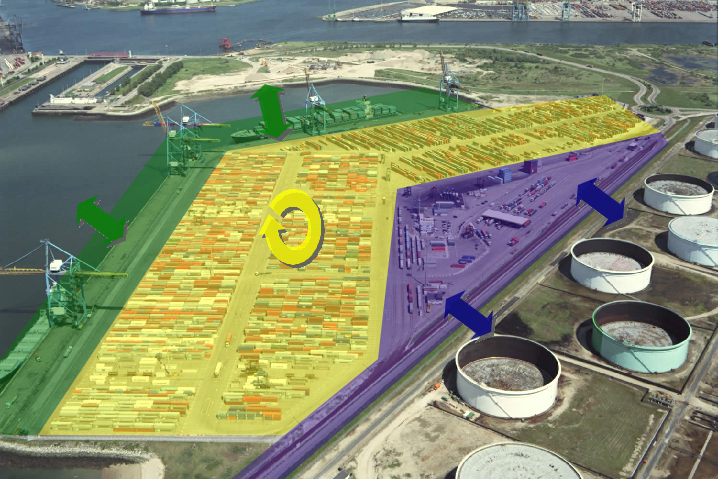
\includegraphics[height=.5\textheight]{fig/threeKindsOfMissions.png}
	\end{flushright}
  \end{column}
\end{columns}
\end{frame}


\begin{frame}
\subsection*{Les chariots cavaliers} 
\frametitle{Les chariots cavaliers}
\begin{columns}
  \begin{column}[l]{8cm}
    \begin{itemize}
    \item Les chariots cavaliers sont des engins de manutention qui peuvent transporter un conteneur à la fois
    \item Ils sont capables d'enjamber une travée de conteneurs et de prendre (déposer) un conteneur sur le sommet d'une pile
    \item Une mission consiste à déplacer un conteneur d'un point $A$ à un point $B$ sur le terminal
    \end{itemize}
  \end{column}
  \begin{column}[r]{3cm}
	\begin{flushright}
	    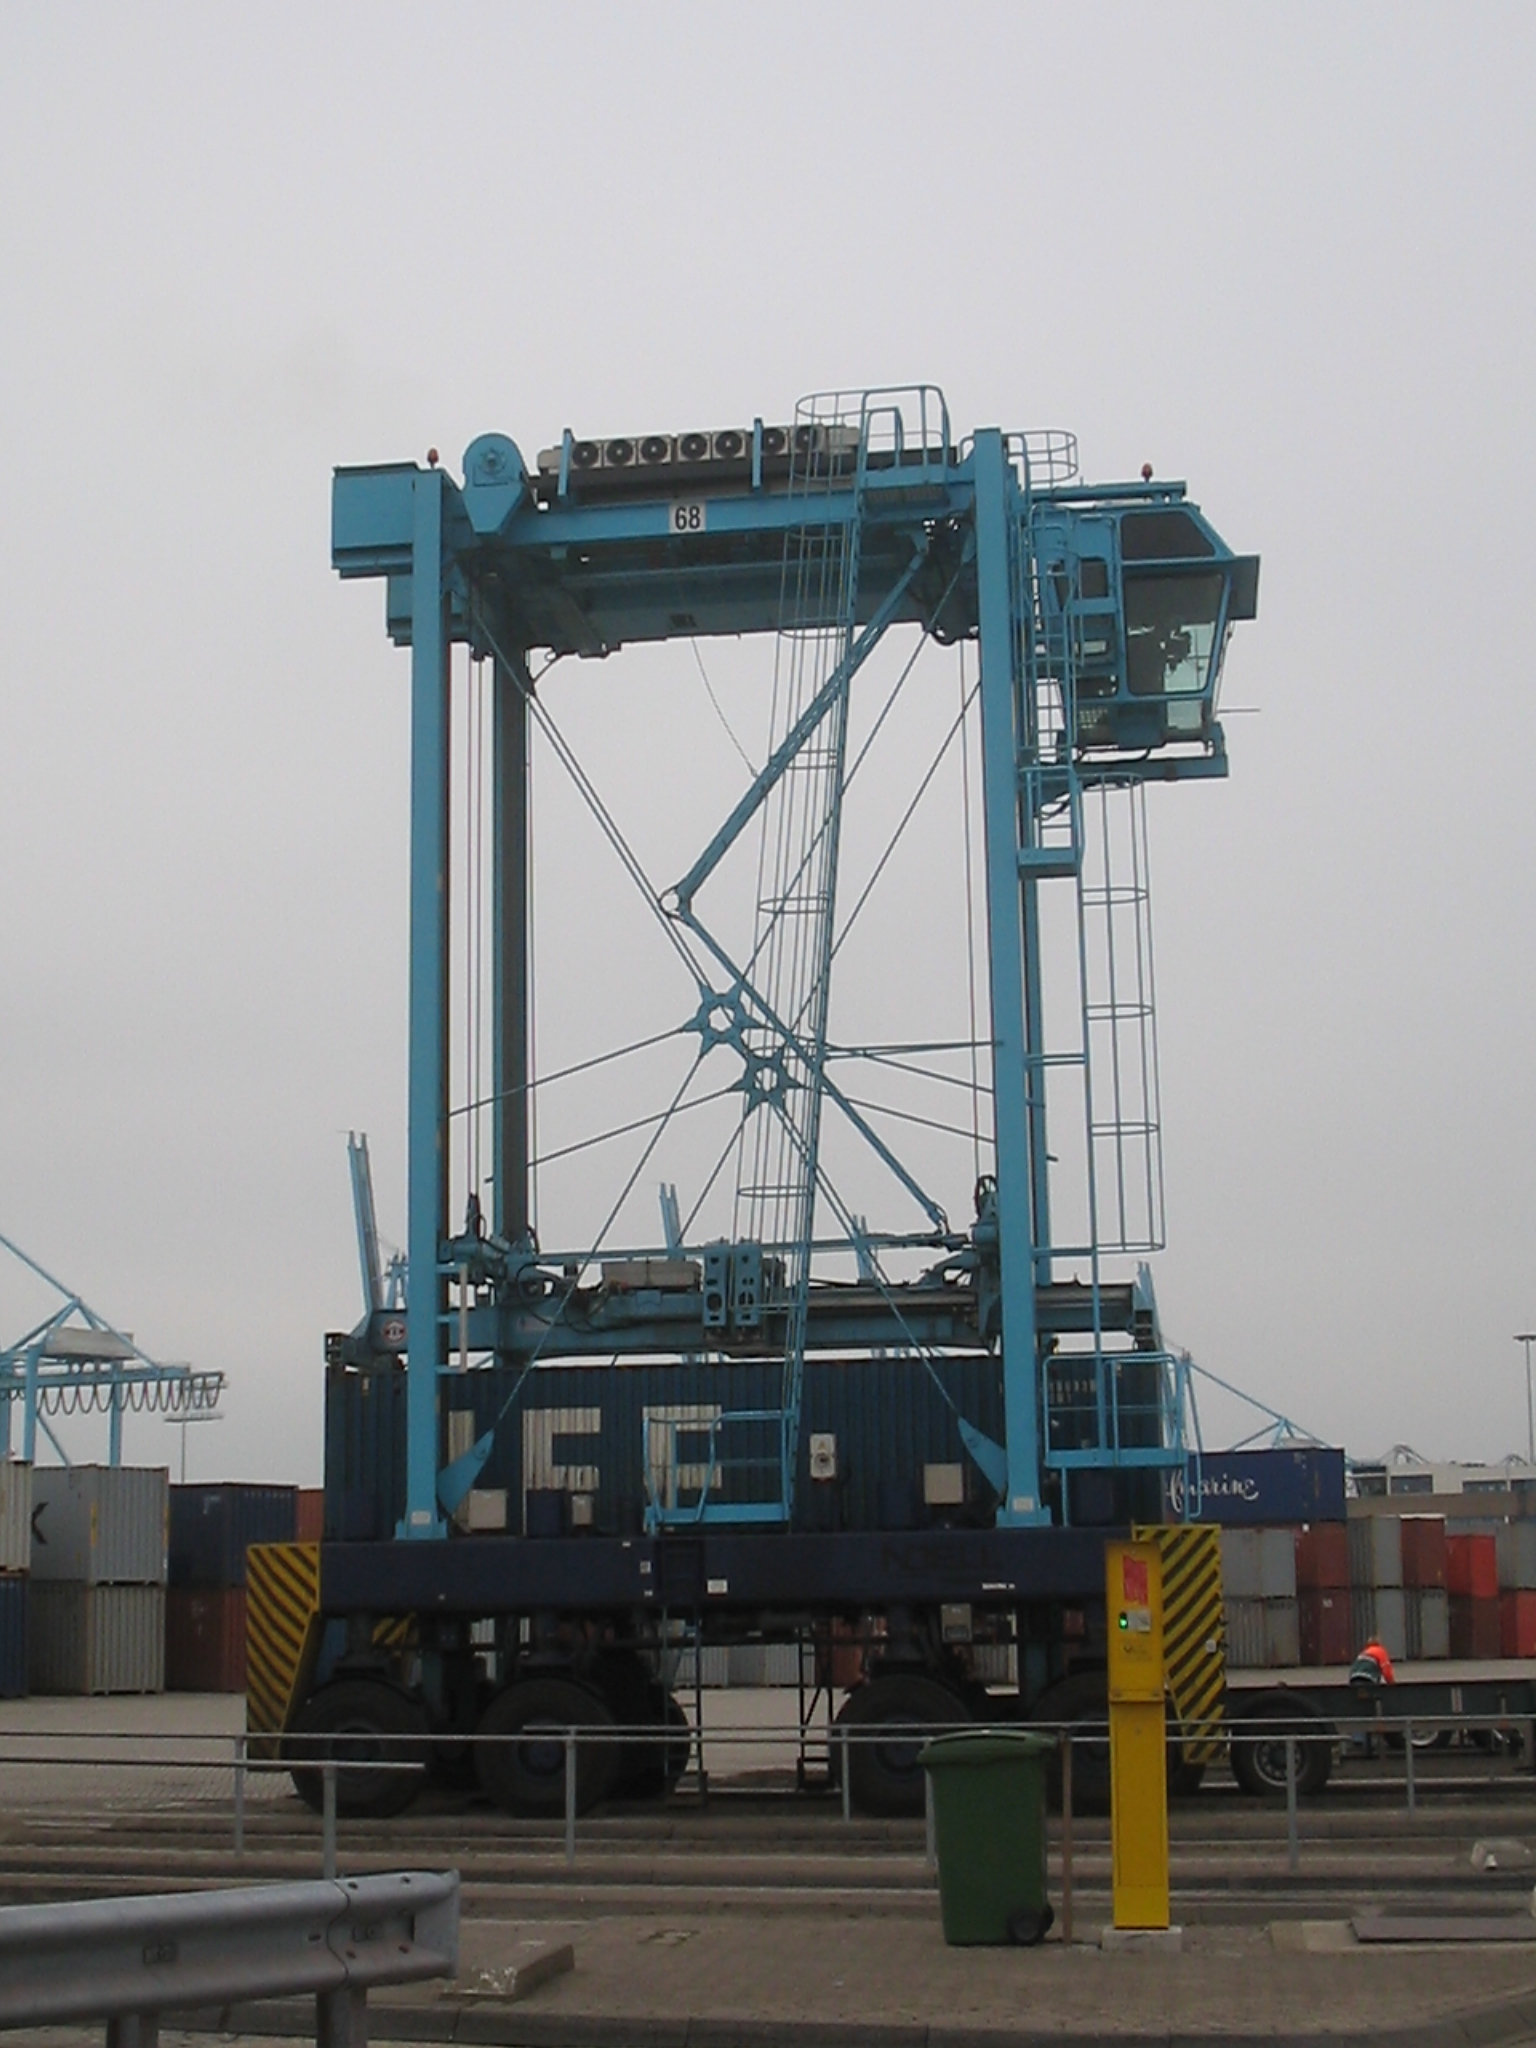
\includegraphics[height=.5\textheight]{fig/Containerlift_straddle_carrier.jpg}
	\end{flushright}
  \end{column}
\end{columns}	
\end{frame}

\subsection*{Dynamicité du système}
\begin{frame}
\frametitle{Système ouvert}
	\begin{columns}
		\begin{column}[l]{8cm}
			Un système ouvert implique un environnement incertain.

			Les flots entrants et sortants : 
			\begin{itemize}
				\item ne dépendent pas uniquement du système lui-même
				\item affectent le système et le conduisent dans un nouvel état
			\end{itemize}
		\end{column}
		\begin{column}[r]{4cm}
			\begin{center}
				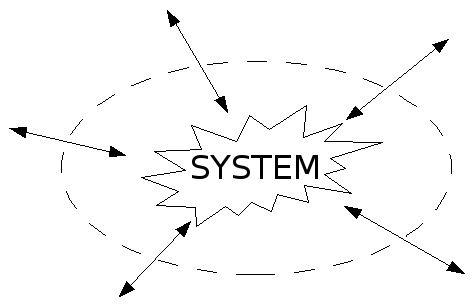
\includegraphics[height=.30\textheight]{fig/openSystem.png}
			\end{center}
	 	\end{column}
	\end{columns}
\end{frame}
\begin{frame}
\frametitle{Environnement incertain}
	Il existe plusieurs événements imprévisibles tels que :
	  \begin{itemize}
	  \item L'arrivée des missions
	  \item L'heure d'arrivée des camions, des  trains, et des navires
	  \item Les déconnections au sein du réseau routier (et ferroviaire)
	  \item Les pannes des engins de manutention
	  \item Le comportement humain
	\end{itemize}
\end{frame}

\section{Optimisation du terminal}
\begin{frame}
\subsection*{Le projet CALAS}
\frametitle{Le projet CALAS}
\begin{columns}
    \begin{column}[l]{4.9cm}	
	\begin{itemize}
		\item Système de mesure laser
		\item Principales entreprises :
		    \begin{itemize}
			\item LDTT
			\item EADS
		    \end{itemize}
		\item Principaux laboratoires :
			 \begin{itemize}
			    \item LMAH
			    \item LITIS
			  \end{itemize}
	\end{itemize}
    \end{column}
    \begin{column}[r]{5cm}
		\begin{flushright}
		  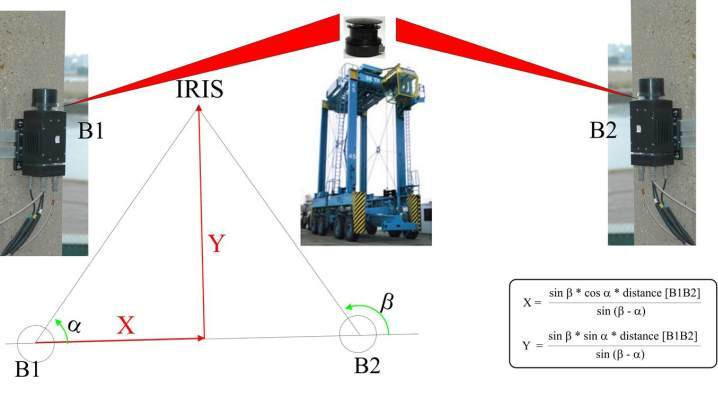
\includegraphics[height=.37\textheight]{fig/angles.jpg}
		\end{flushright}
    \end{column}
 \end{columns}	
	\begin{block}{Objectifs du projet CALAS : }
		\begin{minipage}[]{\columnwidth}
			Connaître l'état du terminal en temps réel, c'est-à-dire à la fois la position des conteneurs et celle des engins de manutention.
		\end{minipage}
	\end{block}
\end{frame}

\begin{frame}
\subsection*{Ordonnancement robuste des missions}
\frametitle{Ordonnancement dynamique\cite{lesauvageICCSA2009,lesauvageMajestic09}}
%Notre approche :
\begin{block}{Ordonnancement des missions par intelligence collective : }
  \begin{itemize}    
    \item Les missions à ordonnancer forment un graphe orienté    
    \item Une colonie de fourmis pour chaque véhicule
    \item Coloration de graphe par mécanismes de collaboration/compétition\cite{bertelle02}
  \end{itemize}
\end{block}

  
\begin{block}{Avantages : }
  \begin{itemize}
    \item Robustesse : tout événement modifie le graphe et donc modifie également le comportement des fourmis
    \item Anytime : une solution est disponible à tout moment
    \item Bien adapté à la nature dynamique du problème et à l'incertitude
  \end{itemize}
\end{block}


\end{frame}

\begin{frame}
\subsection*{Routage des chariots cavaliers}
\frametitle{Routage des chariots cavaliers}

\begin{itemize}
 \item Les chariots peuvent se doubler et se croiser sur une même route
 \item Les chariots ne peuvent ni se doubler ni se croiser dans une travée
\end{itemize}

\begin{itemize}
 \item Les travées sont des arcs/arêtes FIFO alors que les routes sont non FIFO
 \item Il est important de prendre en compte le temps d'attente en entrée de travée dans le routage des chariots cavaliers\cite{Orda90}
 \end{itemize}


\end{frame}

\section{Simulateur}
\begin{frame}
\frametitle{Simulateur de terminal portuaire à conteneurs}
 \begin{block}{Objectifs : }
    \begin{itemize}
     \item Permettre de tester les modèles développés pour optimiser le fonctionnement du terminal
    \end{itemize}
 \end{block}
  \begin{block}{Moyens : }
   \begin{itemize}
     \item Reproduire la structure et le comportement d'un terminal
     \item Gérer la dynamique du système
   \end{itemize}
  \end{block}

  \begin{block}{Technologies utilisées : }
    \begin{itemize}
     \item Java
     \item RMI
     \item GraphStream\cite{graphstream}
    \end{itemize}
  \end{block}
\end{frame}

\tiny
\bibliographystyle{plain}
\bibliography{biblioReunionProjetPassagePortuaire}
\end{document}